\section{Optimization model and solution strategy}\label{sec:OptimizationModel}
%
This section presents the optimization problem. The rest of this section is organized as follows. First, the time sequence of decisions for participation in the mFRR market is presented. Second, we explain how scenarios for price data are generated. Third, we present the model formulation. Fourth, we discuss how the bidding policy is implemented. Lastly, we show how a scenario decomposition method with an ADMM strategy is used to solve the optimization model with up to 250 scenarios.

\vspace{-1mm}
\subsection{Time sequence for decision making}
Fig. \ref{fig:timeline_mfrr_variables} shows the stages for making decisions in the mFRR market. In the first stage in day $\rm{D}$-1, the BRP makes a reservation bid decision $p_{h}^{\rm{r},\uparrow}$ for every hour $h$ of day $\rm{D}$,  while being uncertain about input parameters in the next three stages including day-ahead market clearing, mFRR activation bid, and real time. For simplicity and avoid the need for developing a multi-stage stochastic program, we merge all the three stages as one, and call it the second stage. By this, $p_{h}^{\rm{r},\uparrow}$ is the first-stage variable, whereas the second stage variables, indexed by scenario $\omega$, include
the regulating power bid $\lambda_{h,\omega}^{\text{bid}}$ and the set $\Gamma_{\omega}$ containing all real-time variables. Variables in $\Gamma_{\omega}$ include the real-time power activated, as well as auxiliary variables for identifying up- and down-regulation,  temperature dynamics, and when to deliver up-regulation according to the bid and prices (see Appendix A for a detailed description). Note that down-regulation refers to the rebound action in this context.
% \begin{figure}[!t]\label{fig:timeline_mfrr_variables}
%     \centering
%     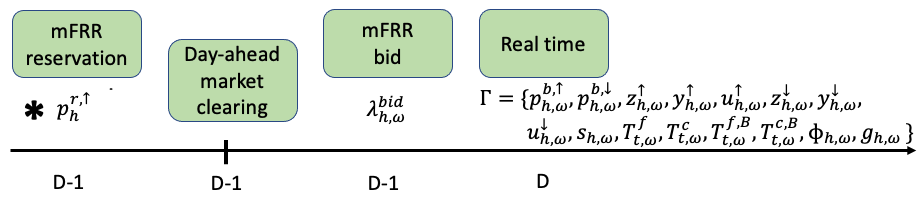
\includegraphics[width=\columnwidth]{../figures/timeline_mfrr_variables.png}
%     \caption{Variables related to mFRR up-regulation decisions. The asterisk indicates the first-stage decision.}
% \end{figure}

\begin{figure}[b]
    \centering
    \includestandalone[width=\columnwidth]{../figures/timeline_mfrr_variables_tikz}
    \caption{Variables related to the mFRR  decisions. The asterisk indicates the first-stage variable.  The variable $\bm{\lambda}_{\omega}^{\text{bid}}$ as well as the set $\Gamma_{\omega} = \{ \bm{p}^{\rm{r},\uparrow}$, $\bm{p}_{\omega}^{\rm{b},\uparrow}$, $\bm{p}_{\omega}^{\rm{b},\downarrow}$, $\bm{s}_{\omega}$, $\bm{T}_{\omega}^{\rm{c}}$, $\bm{T}_{\omega}^{\rm{f}}$, $\bm{T}_{\omega}^{\rm{c,B}}$, $\bm{T}_{\omega}^{\rm{f,B}}$, $\bm{\phi}_{\omega}$, $\bm{g}_{\omega} \}$ are the second-stage  variables.}
    \label{fig:timeline_mfrr_variables}
\end{figure}

\vspace{-1mm}
\subsection{Scenario generation}\label{sec:scenario_generation}
To obtain an efficient policy for making decisions on reservation capacity $p_{h}^{\rm{r},\uparrow}$ and regulating power bid $\lambda_{h,\omega}^{\text{bid}}$, we generate a set of scenarios $\omega \in \Omega$ for  mFRR and day-ahead (spot) price data, such that each scenario contains price data for the entire day in question. We refer to them as \textit{in-sample} scenarios. We use two different strategies for in-sample scenario generation: (\textit{i}) considering historical Danish prices in 2021, with different cases where the number of scenarios $|\Omega|$ is 1, 5, 10, 20, 30, 40, 50, 100, and 250. (\textit{ii}) considering prices of the most recent five days (lookback strategy). In both scenario generation strategies, balancing prices $\lambda_{h,\omega}^{\rm{b}}$ are sampled in the following way: First, an integer $x$ is sampled uniformly from $\{0, \ldots, 24\}$ which represents the total number of up-regulation hours in a day. We then sample price differentials, i.e., $\bm{\lambda}^{\rm{b}}-\bm{\lambda}^{\rm{s}}$, from a single day within the set of all days where up-regulation happened $x$ times. This constitutes one scenario and is repeated $|\Omega|$ times. In this way, days where up-regulation happened are essentially up-sampled, and the model learns more when up-regulation happens than otherwise. The in-sample results are systematically compared against the same set of unseen \textit{Out-of-Sample} (OOS) scenarios, which are Danish prices for 2022.

For load shifting, the solution approach is simply to solve a deterministic optimization problem for the next day, since the day-ahead (spot) market clearing happens in advance, and thereby the spot prices are known.

\vspace{-1mm}
\subsection{Model formulation}
Aligned with \eqref{eq:mFRRObjective} but in a two-stage stochastic setting, the objective function of a BRP offering mFRR services to maximize her expected profit is
%
\begin{subequations}\label{P1:compact_model}
    \begin{align}
        \underset{\bm{p}^{\rm{r},\uparrow}, \bm{\lambda}_{\omega}^{\text{bid}}, \bm{\Gamma}_{\omega}}{\textrm{max}} \quad & f(\bm{p}^{\rm{r},\uparrow}) + \sum_{\omega \in \Omega} \pi_{\omega} g(\bm{\Gamma}_{\omega}) \label{P1:eq1}
        \\
        \text{s.t.} \quad                                                                                                 & h(\bm{p}^{\rm{r},\uparrow}, \bm{\lambda}_{\omega}^{\text{bid}}, \bm{\Gamma}_{\omega}) \leq 0, \quad \forall{\omega}\label{P1:eq2}                                                                                        \\
        \quad                                                                                                             & \text{State-space model } (\ref{eq:2ndFreezerStateSpace}), \quad \forall{\omega} \label{P1:eq3}
        \\
        \quad                                                                                                             & \Bigl( \bm{p}^{\rm{r},\uparrow}, \bm{\lambda}_{\omega}^{\text{bid}}, \bm{p}_{\omega}^{\rm{b},\uparrow}, \bm{p}_{\omega}^{\rm{b},\downarrow}, \bm{s}_{\omega}, \bm{T}_{\omega}^{\rm{c}}, \bm{T}_{\omega}^{\rm{f}}, \notag \\ \quad & \quad \bm{T}_{\omega}^{\rm{c,B}}, \bm{T}_{\omega}^{\rm{f,B}}, \bm{\phi}_{\omega}, \bm{g}_{\omega} \Bigr) \in \mathbb{R}^{n}  \label{P1:eq4}
        \\
        \quad                                                                                                             & \bm{u}_{\omega}, \bm{z}_{\omega}, \bm{y}_{\omega} \in \{0,1\},  \label{P1:eq5}
    \end{align}
\end{subequations}
%
where $\pi_{\omega}$ is the probability assigned to in-sample scenario $\omega$. Constraint (\ref{P1:eq2}) incorporates activation of the bid, whereas (\ref{P1:eq3}) models temperature dynamics in the freezer. Constraints (\ref{P1:eq4})-(\ref{P1:eq5}) declare continuous and binary variables, respectively. Note that \eqref{P1:compact_model} is a MILP problem.


For optimal decision making for load shifting, \eqref{P1:compact_model} is simplified by removing scenarios as well as reservation and bid constraints, and replacing the objective function (\ref{P1:eq1}) by minimizing the total power purchase cost $\bm{\lambda}^{\rm{s}} \bm{p}$.

\vspace{-1mm}
\subsection{Regulating power bidding implementation}\label{sec:mFRR_bidding_implementation}
Recall from  Fig. \ref{fig:timeline_mfrr_variables} that we have merged two stages making regulating power bidding decisions $\bm{\lambda}_{\omega}^{\text{bid}}$ and real-time operational decisions $\Gamma_{\omega}$ in one. This is the reason both set of variables $\bm{\lambda}_{\omega}^{\text{bid}}$ and $\Gamma_{\omega}$ are similarly indexed by $\omega$, while in reality, the decision $\bm{\lambda}_{\omega}^{\text{bid}}$ should be made before $\Gamma_{\omega}$. This also challenges the ex-post OOS simulation. To resolve it, we use a learning policy, such that we replace scenario-indexed variable $\lambda_{h,\omega}^{\text{bid}}$ in \eqref{P1:compact_model} by
%
\begin{align}\label{eq:affine_policy}
     & \alpha ( \lambda_{h+1,\omega}^{\rm{s}} - \lambda_{h,\omega}^{\rm{s}}) + \beta + \lambda_{h,\omega}^{\rm{s}}, \quad \forall{\omega}, \forall{h} \in \{1, \ldots, 23\},
\end{align}
where $\alpha$ and $\beta$ are first-stage non-negative variables --- they are not indexed by $\omega$. Indeed, this replacement shrinks the degree of freedom for the BRP compared to \eqref{P1:compact_model}, but makes it more practical to be used. By this trick, the regulating power bidding decision to be made at 5pm of day $\rm{D}$-1 (see Fig. \ref{fig:timeline_mfrr_variables}) becomes a first-stage decision, dependent not only on policies $\alpha$ and $\beta$, but also on uncertain spot prices $\lambda_{h,\omega}^{\rm{s}}$. In other words, by using the in-sample scenarios $\omega$, the BRP obtains optimal values for $\alpha$ and $\beta$ at 9:30am of day $\rm{D}$-1. Then, she waits to see the spot prices at noon of day $\rm{D}$-1, and then submits her regulating power bids, following \eqref{eq:affine_policy}, at 5pm of day $\rm{D}$-1.

The rationale behind the way we define \eqref{eq:affine_policy} is as follows: a flexible demand would ideally like to up-regulate in hours where subsequent hours have lower spot prices. Thus, the rebound is more likely to be less costly. \red{unfortunately, I lost your text. Could you please write why we define (5) in a differential way?}

%To solve Problem (\ref{P1:compact_model}), we first need to specify a bidding policy that can readily be used OOS. We do so by choosing an affine bidding policy. Afterwards, it is shown how the bidding policy is implemented using McCormick relaxation.

%\subsubsection{Affine bidding policy}

%A bidding policy needs to be easy to follow OOS for the trader. We choose an affine bidding policy, i.e., a linear function of the spot price. The bidding policy is given by:





%Variables $\alpha$ and $\beta$ are then learned IS and fixed for OOS evaluation. After the day-ahead market clearing, (\ref{eq:affine_policy}) can easily be used to specify bids for the next day.

Another implementation challenge is to enforce price conditions under which the accepted mFRR reservation can be activated.
Recall from Section \ref{sec:mFRR}, for the activation, it is necessary to hold $ \bm{\lambda}^{\text{bid}} <  \bm{\lambda}^{\rm{b}}$ and $ \bm{\lambda}^{\rm{b}} > \bm{\lambda}^{\rm{s}}$. This is challenging, because making a condition on variable $ \bm{\lambda}^{\text{bid}}$ imposes non-linearity. These conditions can be equivalently enforced as
%
%activation of mFRR reservation only happens when certain price conditions are met. This is formalized in the following constraint:
%
\begin{equation}\label{eq:bid_constraint}
    p^{\rm{b}, \uparrow}_{h,\omega} + s_{h,\omega} \geq p^{\rm{r},\uparrow}_{h}  \mathbbm{1}^{\big(\lambda^{\text{bid}}_{h,\omega} < \lambda^{\rm{b}}_{h,\omega} \ \text{and} \ \lambda^{\rm{b}}_{h,\omega} > \lambda^{\rm{s}}_{h,\omega}\big)}, \quad \forall{h,\omega},
\end{equation}
where $\mathbbm{1}^{(.)}$ is 1 if conditions (.) are met, otherwise it is zero. If the non-negative slack variable $s_{h,\omega}$ takes a non-zero value, it shows the BRP fails in the activation stage, and therefore will be penalized. To linearize \eqref{eq:bid_constraint}, we use a McCormick relaxation \cite{mccormick1976computability} to define auxiliary continuous variable $\phi_{h,\omega} \in \mathbb{R}$ and $g_{h,\omega} \in \{0, 1\}$, and eventually replace \eqref{eq:bid_constraint} by a set of mixed-integer linear constraints as
%
%Eq. (\ref{eq:bid_constraint}) shows how real-time up-regulation plus a slack variable must be greater than or equal to the reservation if the bid is lower than the balancing price and if up-regulation is needed in hour $h$. It is a bi-linear constraint so McCormick relaxation \cite{mccormick1976computability} is used to convert (\ref{eq:bid_constraint}) to a linear constraint by introducing auxiliary variables, $\phi_{h,\omega}$ and $g_{h,\omega}$:
%
\begin{subequations}\label{eq:bid_constraint_relaxed}
    \begin{align}
        \lambda_{h,\omega}^{\rm{b}} - \lambda_{h}^{\rm{s}} \geq \lambda_{h,\omega}^{\rm{bid}} - M  (1 - g_{h,\omega}) , \quad                        & \forall{h,\omega}             \label{con_bid:subeq1}  \\
        \lambda_{h,\omega}^{\rm{bid}} \geq \lambda_{h,\omega}^{\rm{b}} - \lambda_{h}^{\rm{s}} - M  (1 - g_{h,\omega}) , \quad                        & \forall{h,\omega}             \label{con_bid:subeq2}  \\
        p^{\rm{b}, \uparrow}_{h,\omega} \leq \phi_{h,\omega}  \mathbbm{1}^{\lambda^{\rm{b}}_{h,\omega} > \lambda^{\rm{s}}_{h}}, \quad                & \forall{{h,\omega}}           \label{con_bid:subeq3}  \\
        p^{\rm{b}, \uparrow}_{h,\omega} + s_{h,\omega} \geq \phi_{h,\omega}  \mathbbm{1}^{\lambda^{\rm{b}}_{h,\omega} > \lambda^{\rm{s}}_{h}}, \quad & \forall{{h,\omega}}           \label{con_bid:subeq4}  \\
        -g_{h,\omega}  M \leq \phi_{h,\omega}, \quad                                                                                                 & \forall{h,\omega}             \label{con_bid:subeq5}  \\
        \phi_{h,\omega} \leq g_{h,\omega}  M, \quad                                                                                                  & \forall{h,\omega}             \label{con_bid:subeq6}  \\
        -(1 - g_{h,\omega})  M \leq \phi_{h,\omega} - p^{\rm{r},\uparrow}_{h}, \quad                                                                 & \forall{h,\omega}             \label{con_bid:subeq7}  \\
        \phi_{h,\omega} - p^{\rm{r},\uparrow}_{h} \leq (1 - g_{h,\omega})  M, \quad                                                                  & \forall{h,\omega},             \label{con_bid:subeq8}
        % \lambda_{h,\omega}^{\rm{bid}} \leq \lambda^{Max} \label{con_bid:subeq9}
    \end{align}
\end{subequations}
where $M$ is a large enough positive constant.
Constraints \eqref{con_bid:subeq1}-\eqref{con_bid:subeq2} ensure that $g_{h,\omega} = 1$ when the balancing price minus the spot price is larger than the regulating power bid $\lambda^{\rm{bid}}_{h, \omega}$, and zero otherwise. Constraints \eqref{con_bid:subeq3}-\eqref{con_bid:subeq4} set the TCL up-regulation equal to $\phi_{h,\omega}$ (or incurs a penalty through $s_{h,\omega}$) if there is an up-regulation event in the system, i.e., if $\mathbbm{1}^{\lambda^{\rm{b}}_{h,\omega} > \lambda^{\rm{s}}_{h}} = 1$. Constraints \eqref{con_bid:subeq5}-\eqref{con_bid:subeq6} enforce  $\phi_{h,\omega} = 0$ when $g_{h,\omega} = 0$, i.e., when the balancing price differential is smaller than the power regulating bid. Constraints \eqref{con_bid:subeq7}-\eqref{con_bid:subeq8} ensure that $\phi_{h,\omega}$ is equal to the reservation capacity $p^{\rm{r},\uparrow}_{h}$ whenever $g_{h,\omega} = 1$, i.e., if the regulating power bid is smaller than the balancing price differential. Note that in the final model,  $\lambda^{\rm{bid}}_{h, \omega}$ in \eqref{eq:bid_constraint_relaxed} should be replaced as defined in \eqref{eq:affine_policy}. The final model formulation, which is a MILP, is given in Appendix A.

\vspace{-1mm}
\subsection{Scenario decomposition with ADMM}
When solving Problem (\ref{P1:compact_model}) using the first strategy with many scenarios, it quickly becomes computationally intractable due to the number of binaries and intertemporal constraints. To solve it, the ADMM algorithm is used which can solve a large-scale optimization problem by decomposing it into smaller subproblems \cite{boyd2011distributed}. In (\ref{P1:compact_model}), each scenario is solved as a subproblem by setting:

\begin{equation}\label{eq:non_anticipativity}
    \bm{p}^{\rm{r},\uparrow} \rightarrow \bm{p}^{\rm{r},\uparrow}_{\omega}, \quad \alpha \rightarrow \alpha_{\omega}, \quad \beta \rightarrow \beta_{\omega}
\end{equation}

The ADMM algorithm will converge by achieving consensus on first- and second-stage stage decisions in linear problems, but it is only a heuristic for MILPs \cite{hong2016convergence}.
